\documentclass{beamer}

\usepackage{beamerthemesplit}
\usepackage{verbatim}

\usetheme{Pittsburgh}
%\usecolortheme{seagull}
%\usecolortheme{seahorse}
\usecolortheme{beaver}

\usefonttheme{serif}

%\DeclareGraphicsExtensions{.pdf,.png,.jpg}

\newcommand{\snT}{$(S/N)_{\textrm{size}}$}
%\newcommand{\snT}{$\left( \frac{S}{N}\right)_{\textrm{size}}$}
\newcommand{\snflux}{$(S/N)_{\textrm{flux}}$}
%\newcommand{\snflux}{$\left( \frac{S}{N}\right)_{\textrm{flux}}$}

\newcommand{\lensfit}{\texttt{LENSFIT}}
\newcommand{\numba}{\texttt{Numba}}
\newcommand{\python}{\texttt{Python}}
\newcommand{\ngmix}{\texttt{ngmix}}
\newcommand{\shear}{{\bf g}}

\title{Weak Lensing Results from DES}
\author{Erin Sheldon}
\institute{Brookhaven National Laboratory}

% http://texblog.net/latex-archive/plaintex/beamer-footline-frame-number/
% to add the page (frame ) number and not screw up the bottom line
% works for split themes?
\expandafter\def\expandafter\insertshorttitle\expandafter{%
      \insertshorttitle\hfill%
        \insertframenumber\,/\,\inserttotalframenumber}

% suppress navigation bar
\beamertemplatenavigationsymbolsempty

\begin{document}

%\frame{\titlepage}

%\section{Dark Energy}

\frame
{
    \frametitle{Dark Energy}

    \fontsize{9}{0.8\baselineskip}
    \begin{columns}
        \begin{column}{0.5\textwidth}    
            \begin{itemize}
                \item The original story is simple

                \item There are objects whose intrinsic brightness we think we
                    know (type 1a supernovae)

                \item If we know one of these objects is at a given distance we
                    should be able to predict its observed brightness

                \item It turns out this only works if we modify the equations
                    so that the universe is accelerating at late times (long
                    after the big bang, recently) instead of slowing down

                \item Either add a new component, such as a cosmological constant,
                    or modify general relativity

            \end{itemize}
        \end{column}
        \begin{column}{0.5\textwidth}
            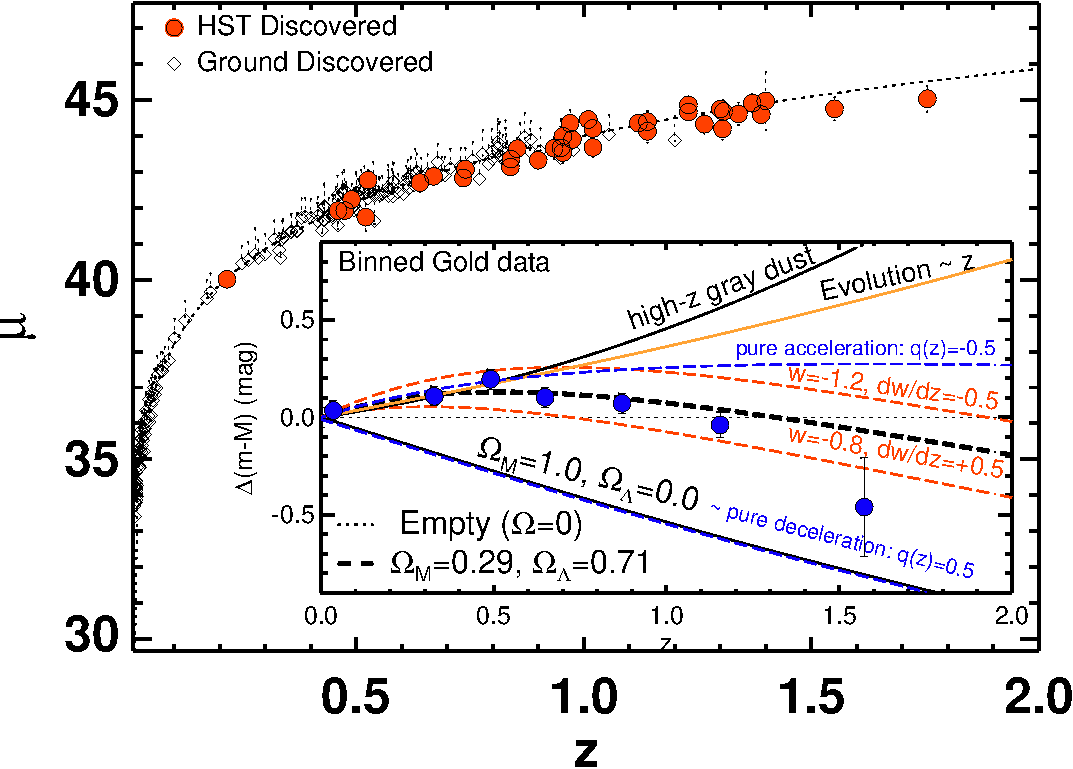
\includegraphics[width=\textwidth]{riess-distmodulus.pdf}
        \end{column}
    \end{columns}
}

\frame
{
    \frametitle{Standard Rulers}

    \fontsize{9}{0.8\baselineskip}
    \begin{columns}
        \begin{column}{0.5\textwidth}    
            \begin{itemize}

                \item The baryon acoustic feature is frozen in when the
                    universe cools enough for baryons and photons to decouple:
                    it is thus a standard ruler

                \item its apparent size at a give distance should be predictable
                    given the observed size in the CMB and a cosmological model.

                \item again, it only works if we modify the equations

            \end{itemize}
        \end{column}
        \begin{column}{0.5\textwidth}
            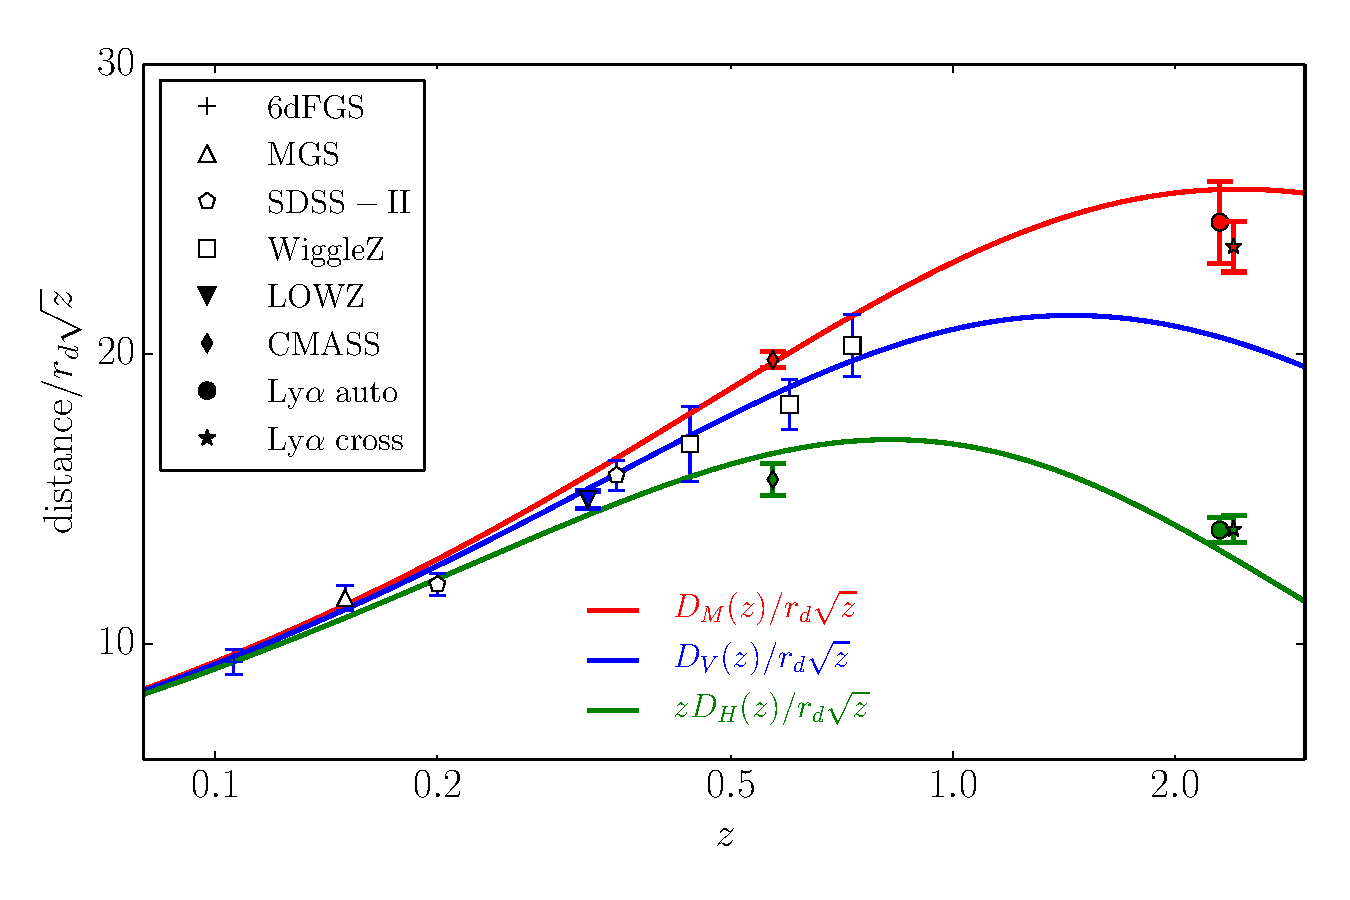
\includegraphics[width=\textwidth]{bao-all.pdf}
        \end{column}
    \end{columns}
}

\frame
{
    \frametitle{Simplest Possible Components}

    \begin{itemize}

        \item Add a constant energy density component to the stress-energy:   A
            cosmological constant $\Lambda$ that has equation of
            state  $p=-\rho$.
            
        \item Constant energy density in an expanding universe is unsatisfying,
            but it matches the data well with our current limited precision.

        \item Next level of complexity: arbitrary equation of state.  This is
            poorly constrained with current data.

    \end{itemize}

    \begin{equation}
        p = w \rho
    \end{equation}

    \begin{itemize}
        \item Any accelerating solution for $w$ ($< - 1/3$) violates the strong energy condition.
    \end{itemize}

}



\frame
{
    \frametitle{Gravitational Lensing}

    \begin{itemize}

        \item Light is apparently deflected as it passes massive bodies.

        \item As with an ordinary lens, the deflection at the detector depends
            on the strength of the lens and the geometry of the
            lens-source-observer system

        \item All objects in the universe are lensed.

        \item We can use this to measure dark matter and dark energy

    \end{itemize}

}

\frame
{
    \frametitle{Lensing Geometry}

    \includegraphics[width=\textwidth]{lens_geometry.pdf}

}

\frame
{
    \frametitle{Example: Lensing Geometry and Dark Energy}

    %\fontsize{9}{0.8\baselineskip}
    \begin{columns}
        \begin{column}{0.5\textwidth}    
            \begin{itemize}

                \item The signal depends on the distance of source behind
                    the lens.

                \item Measure the effect using the same lens and different
                    sources, and try to predict with our cosmological model.

                \item What value of the equation of state $w$ do we need to
                    describe the observations?

            \end{itemize}
        \end{column}
        \begin{column}{0.5\textwidth}
            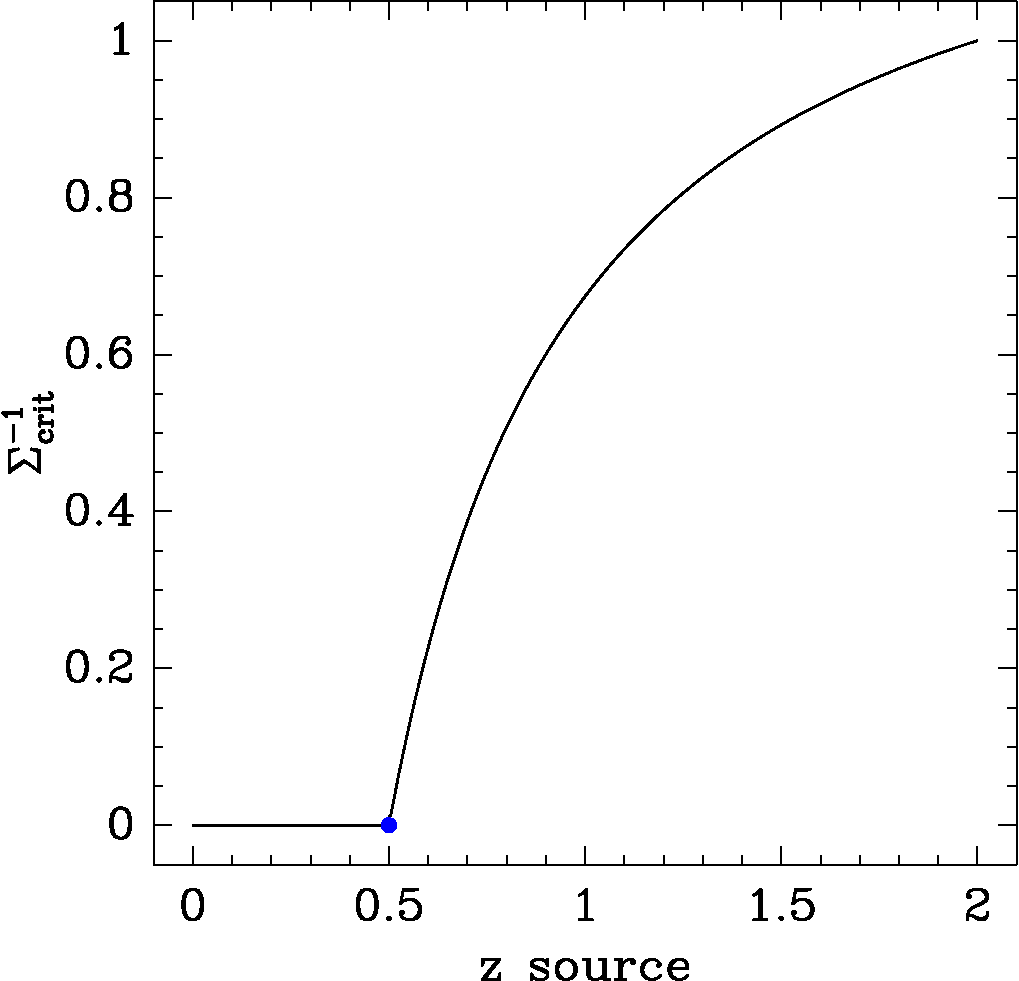
\includegraphics[width=\textwidth]{scinv-example.pdf}
        \end{column}
    \end{columns}
}





%\section{Dark Energy Survey}

\frame
{
    \frametitle{Dark Energy Survey (DES)}

    \fontsize{9}{0.8\baselineskip}
    \begin{columns}
        \begin{column}{0.5\textwidth}    
            \begin{itemize}
                \item Imaging survey of 5000 square degrees in the 
                    southern sky (CTIO) through 5 optical filters.
                \item Study Dark Energy using weak lensing, galaxy clusters, supernovae
                    and large scale structure.
                \item First Light Fall 2012
                \item Survey Start Aug. 31 2013
                \item Erin Sheldon {\bf associate member and builder}; data rights for
                    himself, postdoc, students.
                \item Anders Plazas postdoc working on characterization of detector
                    effects and weak lensing.
            \end{itemize}
        \end{column}
        \begin{column}{0.5\textwidth}
            \includegraphics[width=\textwidth]{ctio_blanco_crew_2013Oct-19-contrast.jpg}
        \end{column}
    \end{columns}
}

\frame
{
    \frametitle{Bayesian Lensing Shear Measurement}

    \begin{columns}
        \begin{column}{0.4\textwidth}
            \begin{itemize}

                \item Figure: Fractional error in the shear for simulated galaxies
                    (exp,dev profiles) near smallest usable {\it observed} size
                    fwhm/fwhm$_{\textrm{psf}}$ = 1.2.

                \item Light Grey: DES requirements
                \item Dark Grey: LSST requirements
            \end{itemize}
        \end{column}
        \begin{column}{0.6\textwidth}
            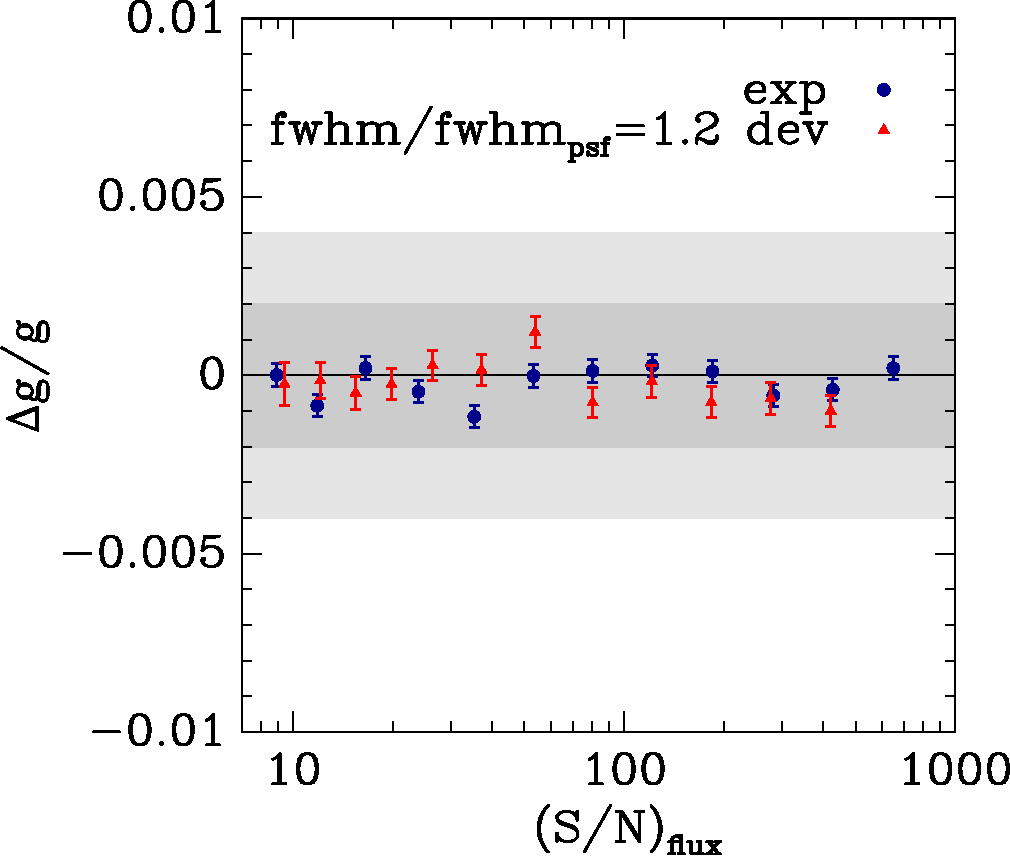
\includegraphics[width=\textwidth]{ngmix-flux-s2n-sigrat-20.pdf}
            \newline

            {\tiny Implementation of recent theoretical work by Bernstein \&
             Armstrong.\par}

        \end{column}
    \end{columns}

}



\end{document}
